%%% Local Variables: 
%%% mode: latex
%%% TeX-master: "tellmemore"
%%% End: 

%results
\begin{figure}[h]
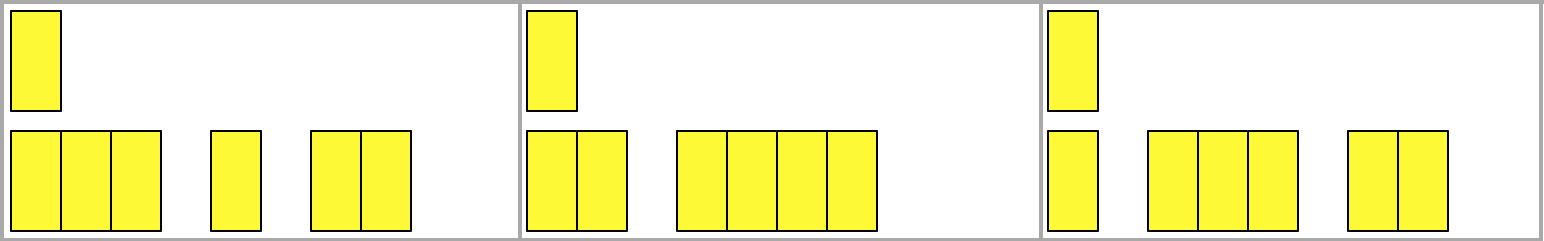
\includegraphics[width = \columnwidth]{./pictures/2_lcs_one/all.png}
\caption{Top results for 2 species full pattern naming game, with similarity scores from left to right of 3, 4, and 4.}
\end{figure} 

\begin{figure}[h]
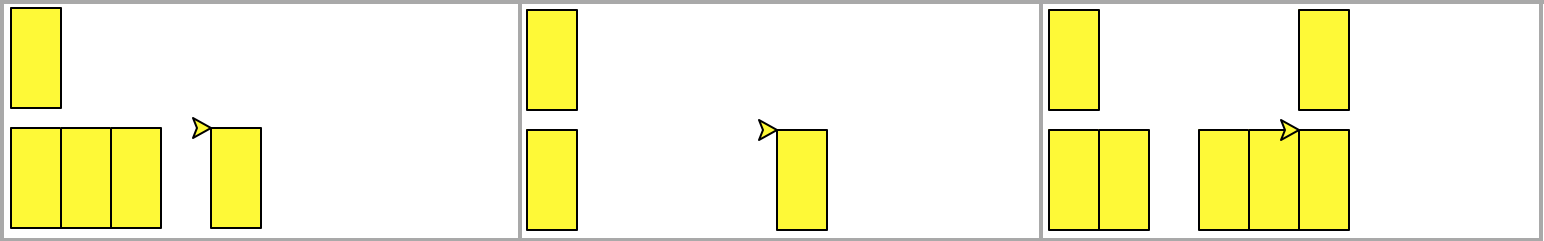
\includegraphics[width = \columnwidth]{./pictures/2_lcs_two/all.png}
\caption{Top results for 2 species partial pattern naming game, with similarity scores from left to right of 7, 9 and 12 .}
\end{figure} 

\begin{figure}[h]
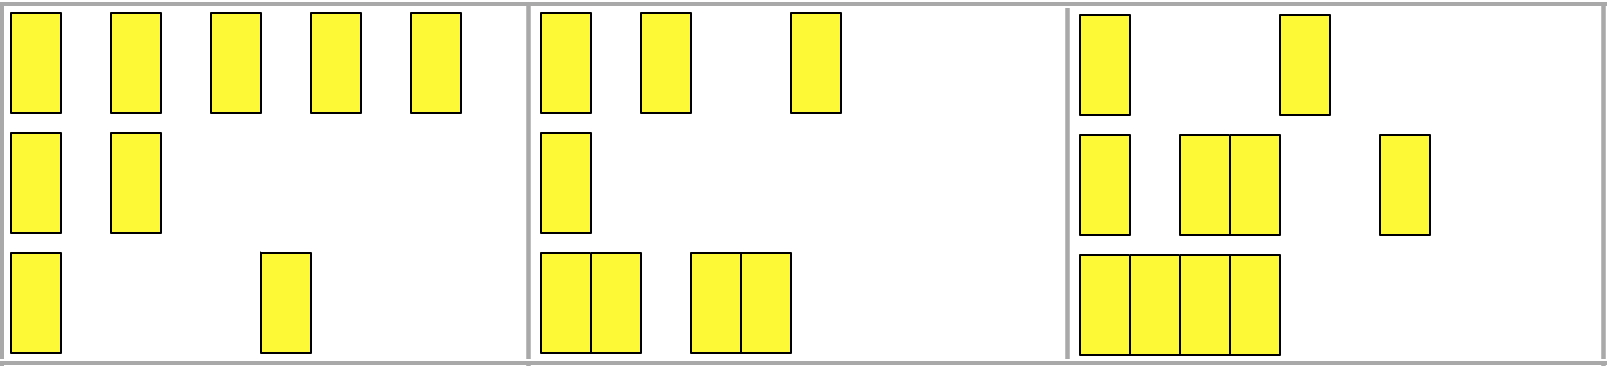
\includegraphics[width = \columnwidth]{./pictures/3_lcs_one/all.png}
\caption{Top results for 3 species full pattern naming game, with similarity scores from left to right of 17.3, 21.7, and 24.}
\end{figure} 

\begin{figure}[h]
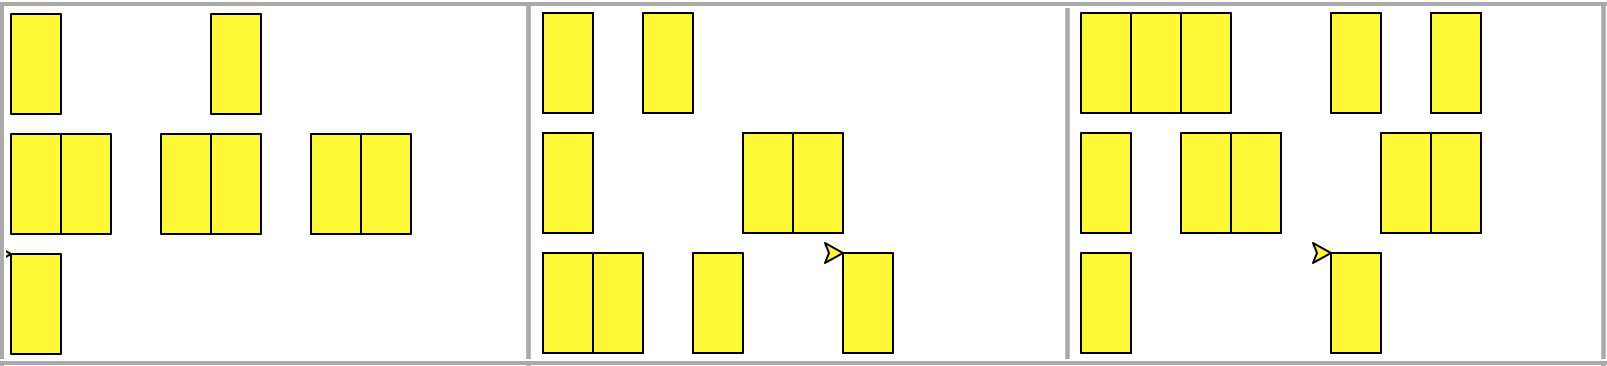
\includegraphics[width = \columnwidth]{./pictures/3_lcs_two/all.png}
\caption{Top results for 3 species partial pattern naming game, with similarity scores from left to right of 18, 24.7, and 25 .}
\end{figure} 

\begin{figure}[h]
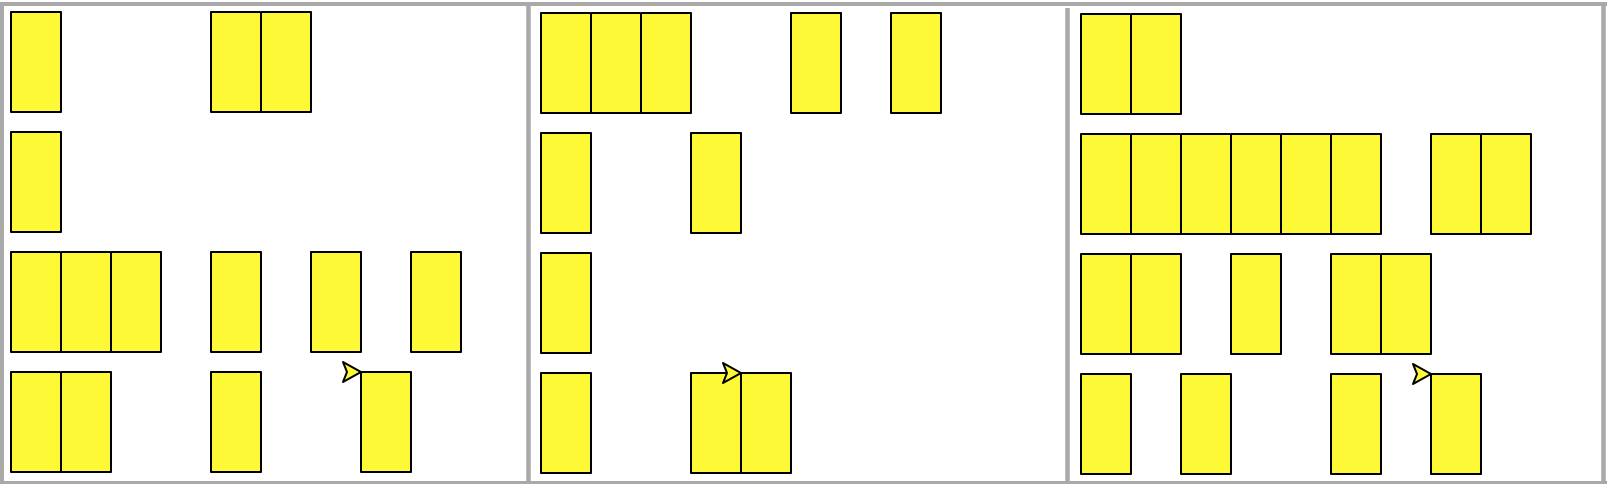
\includegraphics[width = \columnwidth]{./pictures/4_lcs_one/all.png}
\caption{Top results for 4 species full pattern naming game, with similarity scores from left to right of 20.3, 21.3, and 26.3.}
\end{figure} 

\begin{figure}[h]
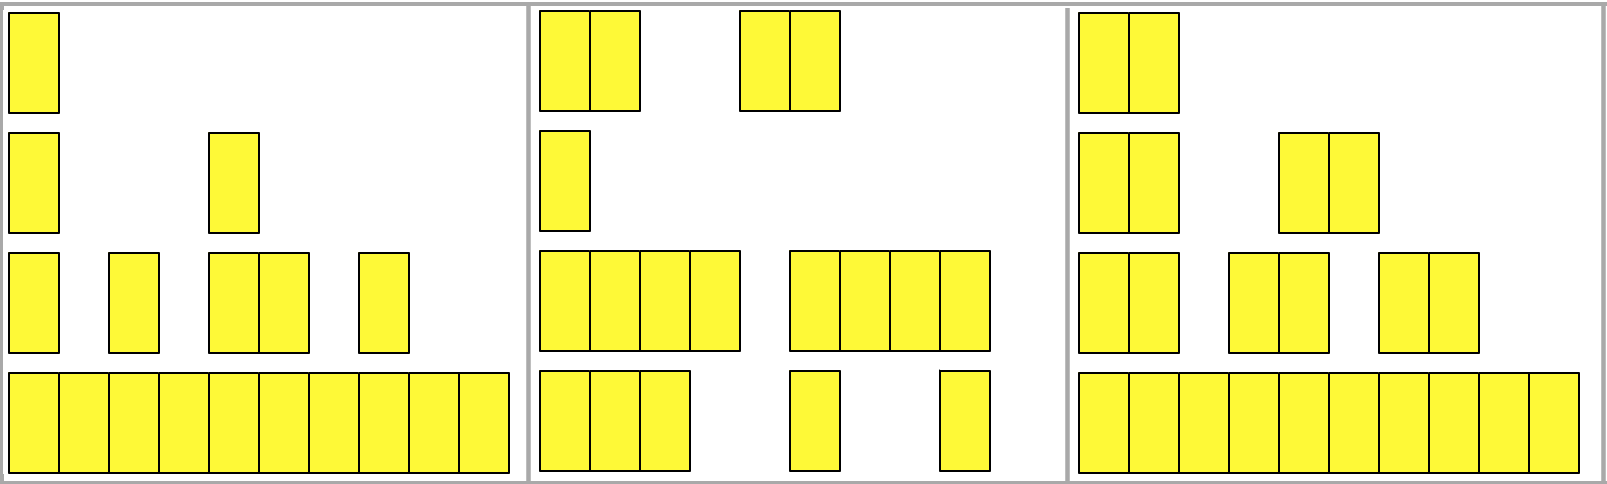
\includegraphics[width = \columnwidth]{./pictures/4_lcs_two/all.png}
\caption{Top results for 4 species partial pattern naming game, with similarity scores from left to right of 16.3, 25, 28.3.}
\end{figure} 

\begin{figure}[h]
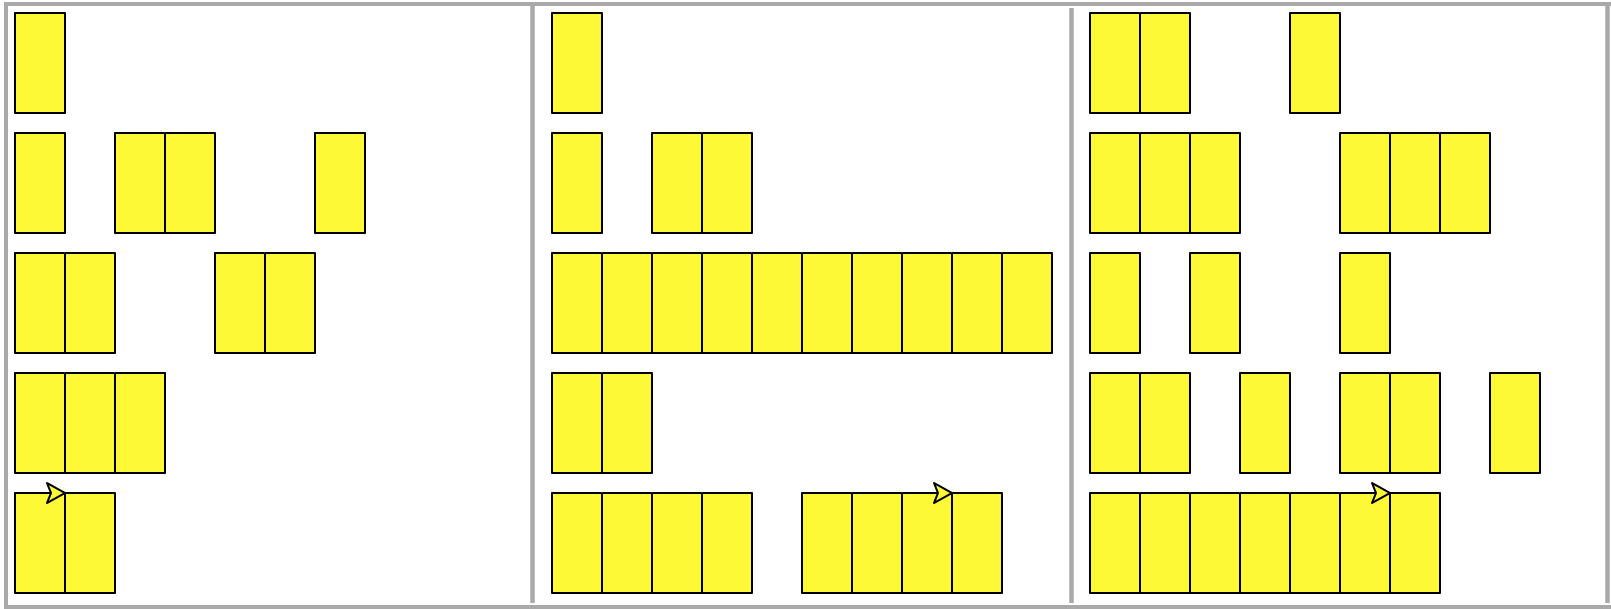
\includegraphics[width = \columnwidth]{./pictures/5_lcs_one/all.png}
\caption{Top results for 5 species full pattern naming game, with similarity scores from left to right of 22.9, 23.1, and 26.3.}
\end{figure} 

\begin{figure}[h]
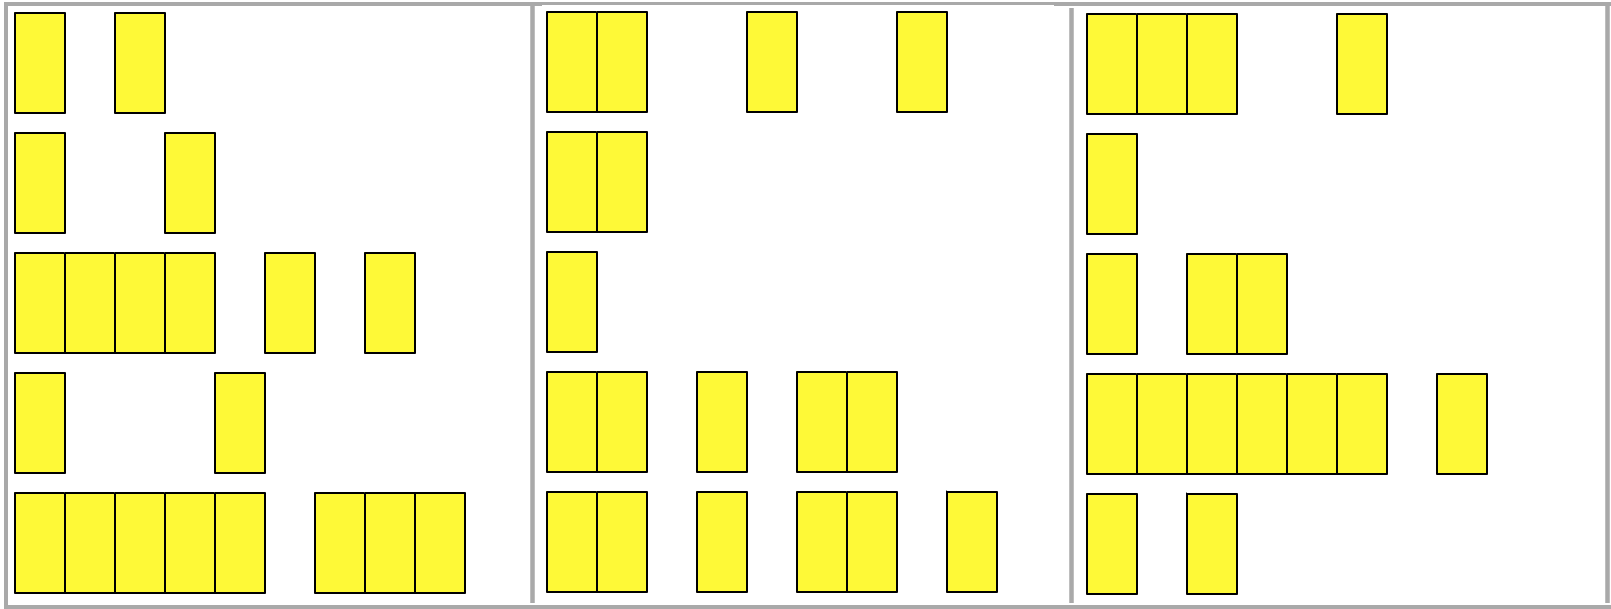
\includegraphics[width = \columnwidth]{./pictures/5_lcs_two/all.png}
\caption{Top results for 5 species partial pattern naming game, with similarity scores from left to right of 24, 25.7, 26.}
\end{figure}  

We experimentally simulated both types of naming games, varying the similarity metric and the number of species.
Each naming game simulation was populated with 15 fireflies of each species and ran for 1000 time steps. 
For each set of parameters, we ran 20 different trials. We present some of the resulting patterns of the trials with the best discounted similarity scores. 

\emph{TODO: we only include lcs metric because...}

For simplicity, we set the pattern length to 10 -- that is, we defined the flash patterns as a sequence of ten 0s or 1s, with a 1 indicating a flash and a 0 indicating no flash for one time unit. 
Because we view the patterns cyclically, there is no inherent starting index with which to present the signals. 
Consequentially, we chose to display the resulting patterns of the naming game as ending with the longest contiguous sequence of 0s, emulating the ``waiting" time observed in firefly signals. When there are two or more sequences of 0s of the same length, we present the patterns starting with the longest contiguous sequence of 1s possible. 

In each figure, we include the resulting patterns from the top three trials of one specification of the naming game. 
Each set of patterns from one trial is contained in its grey bounding box.
Note that the fitness of a flash signal is inherently dependent upon those other patterns with which it evolved, which can be found in the same column. 
We indicate a 1 by a yellow block and a 0 with white space. Contiguous yellow blocks should be interpreted as a single flash of that duration. 

\subsection{Simulations with Two Species}
We use the toy setting of two species to ensure that our similarity metric and rules of the naming game capture our intentions on a basic level.
In the full pattern naming game, we see that one species almost always converges upon the simplest pattern $[1,0,0,0,0,0,0,0,0,0]$, while the other species converges upon patterns with more flashes. We note this tendency to find the simplest pattern as evidence that the naming game instantiates an approximation of our intended selective pressures. 
We see a similar pattern in the partial pattern naming game. Interestingly, the second, more complex patterns, use fewer flashes in general in the partial pattern naming game. 

\subsection{Simulations with More Species}
We then increased the number of species within the simulation up to 5, an upper bound imposed by room to differentiate within the pattern space.
As we increase the number of species within the naming game, it seems that one species is likely to err on the side of more flashes in the trade-off between distinguishability and penalty for flashing, with some opting to keep their flash on at all times. 
While species in simulations with three species seem to be able to manage this trade-off, it seems that as the number of species in the naming game increases, it becomes harder for fireflies to find a distinguishable pattern with low flash cost. 
Indeed, as in most time steps, any one species will have multiple contenders for the final pattern, the search space is quite constrained. 



